\documentclass[serif,8pt]{beamer}
\usetheme{default} % You can change the theme here
\usecolortheme{metropolis} % You can change the color theme here

% Packages for additional functionality
\usepackage{graphicx} % For including images
\usepackage{amsmath} % For mathematical symbols and equations
\usepackage{multirow}
\usepackage{subfig}
\usepackage{braket}
\usepackage{caption}
% \usepackage{authblk}

% /home/bogfootlj/.local/share/fonts/NerdFonts
% Setting up fonts

\graphicspath{{./Images/}} % Where to take images from
\setbeamertemplate{section in toc}[sections numbered]
\setbeamertemplate{subsection in toc}[subsections numbered]

\captionsetup[figure]{labelformat=empty}% redefines the caption setup of the figures environment in the beamer class.
\captionsetup[table]{labelformat=empty}% redefines the caption setup of the figures environment in the beamer class.

% Define the style for the footer with page numbers
\setbeamercolor{footline}{fg=black}
% \addtobeamertemplate{navigation symbols}{}{%
%     \usebeamerfont{footline}%
%     \usebeamercolor[fg]{footline}%
%     \hspace{1em}%
%     \insertframenumber/\inserttotalframenumber
% }

% Define a command to exclude the page counter from the first two slides
\newcommand{\noPageNumber}{%
    \setbeamertemplate{footline}{}%
}

% Define a command to reset the page counter and start numbering from the third slide
\newcommand{\resetPageNumber}{%
    \setbeamertemplate{footline}{%
        \begin{beamercolorbox}[wd=\paperwidth,ht=0.5ex,dp=1ex]{foot}%
            \hspace*{1em}\hfill \insertframenumber/\inserttotalframenumber\hspace*{1em}%
        \end{beamercolorbox}%
    }%
    \addtocounter{framenumber}{-2}
}

% Set up the footer for the rest of the presentation
\setbeamertemplate{footline}{%
    \begin{beamercolorbox}[wd=\paperwidth,ht=0.5ex,dp=1ex]{foot}%
        \hspace*{1em}\hfill%
        \insertframenumber/\inserttotalframenumber\hspace*{1em}%
    \end{beamercolorbox}%
}


% Title slide information
\title{Generating and teleporting entanglement for quantum networks}
\author[Adrian, Rainer]{Adrian Udovičić\\\and Assoc. prof. dr. Rainer Kaltenbaek}
\institute{University of Ljubljana, Faculty of Mathematics and Physics}
\date{23.05.2024, Ljubljana, Slovenia}
\logo{
\includegraphics[height=1cm]{CombinedLogo.png}}

\begin{document}
% Local background must be enclosed by curly braces for grouping.
{\usebackgroundtemplate{\includegraphics[width=\paperwidth,height=\paperheight]{SagnacWithSomeAddedColoursV1.png}}
{\setbeamertemplate{footline}{}

\begin{frame}
	\titlepage
\end{frame}

\usebackgroundtemplate{}
\begin{frame}{Contents and introduction}
  \tableofcontents % Include a table of contents slide
\end{frame}

\resetPageNumber

\section{Motivation}
\usebackgroundtemplate{}
\begin{frame}{Motivation}
  \begin{itemize}
	\item SiQUID
    \item Bright source of entanglement
	\item Training in quantum technologies in Slovenia
	\item Quantum Network for Slovenia
    \item Testbed for industrialized version
	\item Entanglement based QKD
  \end{itemize}
\end{frame}

\section{Theory}
\begin{frame}{Theory}
	\begin{enumerate}
	\item SPDC
	\item Distributing Entanglement
	\end{enumerate}
\end{frame}

\subsection{SPDC}
\begin{frame}{Theory}
	\framesubtitle{SPDC}
		\begin{itemize}
			\item Spontaneous Parametric Downconversion
		\end{itemize}
		\begin{figure}
			\begin{center}
				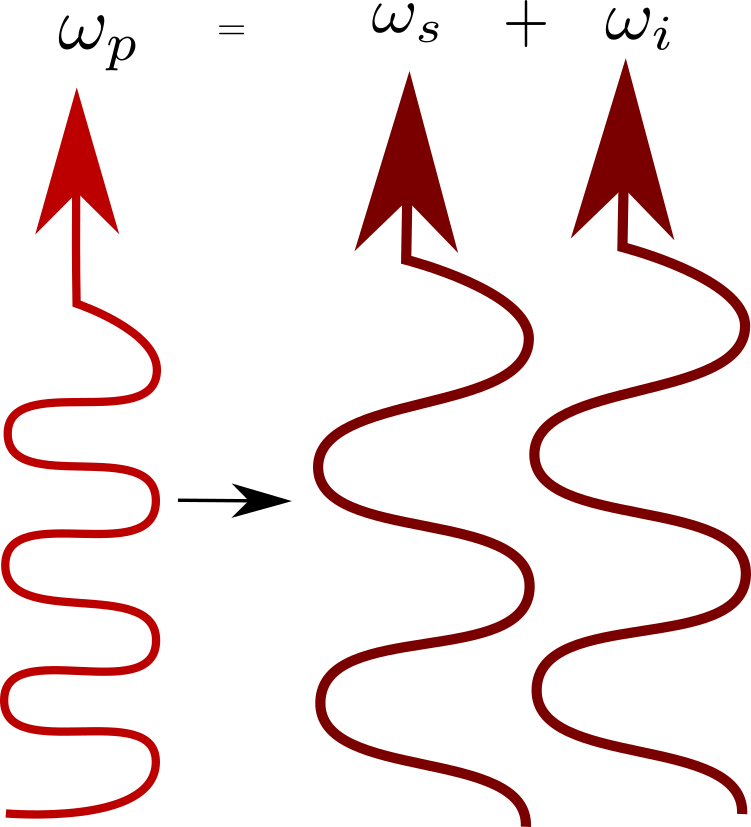
\includegraphics[width=4cm]{SPDC.png}
			\end{center}
			\caption{Illustration of SPDC}\label{fig:SPDC}
		\end{figure}
		\begin{itemize}
			\item Degenerate $\omega_i = \omega_s$
			\item Non-degenerate $\omega_i \ne \omega_s$
		\end{itemize}

\end{frame}

\begin{frame}[t]
	\frametitle{Theory}
	\framesubtitle{State of the Art}
\begin{table}
    \caption{Comparison of different sources}\label{SotA}
    \centering
    \begin{tabular}{|l||l|l|l|l|l|}
        \hline
		& & & & & \\ % Empty line for spacing
        \multirow{2}{*}{\shortstack{Who\\When}}& \multirow{2}{*}{\shortstack{\cite{1}\\2022 }} &\multirow{2}{*}{\shortstack{\cite{2}\\2010 }}  &\multirow{2}{*}{\shortstack{\cite{3}\\2007 }}   & \multirow{2}{*}{\shortstack{\cite{4}\\2006 }}  & \multirow{2}{*}{\shortstack{\cite{5}\\2012 }} \\
		& & & & & \\ % Empty line for spacing
		& & & & & \\ % Empty line for spacing
		% add years
		\hline
        \hline
        Type & 0 & II  & II & II & 0  \\
        \hline
		\multirow{2}{*}{\shortstack{Brightness [$\frac{pairs}{s mW nm}$]}} & \multirow{2}{*}{2,5$\times$$10^6$} & \multirow{2}{*}{87,5$\times$$10^3$} & \multirow{2}{*}{273$\times$$10^3$} & \multirow{2}{*}{5$\times$$10^3$} & \multirow{2}{*}{278$\times$$10^3$}  \\
		& & & & & \\ % Empty line for spacing
        \hline
        Bandwidth [ nm ] & 106 & 0,3  & 0,3 & 1 & 2,3  \\
        \hline
    \end{tabular}
\end{table}
\end{frame}

\subsubsection{Phase Matching}
\begin{frame}
	\frametitle{SPDC}
	\framesubtitle{Phase Matching, Quasi Phase Matching, Bandwidth}
	\begin{itemize}
		\item Birifringent Phase Matching, Quasi Phase Matching
	\end{itemize}

	\begin{figure}
		\begin{center}
		\caption{Illustration of a) Birifringent Phase Matching $k_p = k_i + k_s$ and}
		  \subfloat[][]{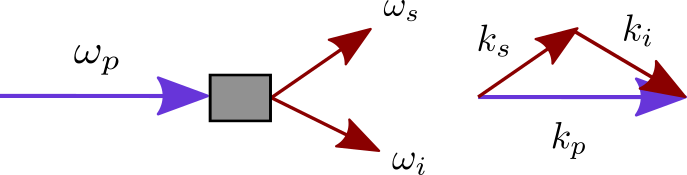
\includegraphics[width=6cm]{SPDCkPM.png}}\\
		  \pause
		\caption{b) Quasi Phase Matching $ k_p - k_i -k_s - \Delta k = 0 $.}
		  \subfloat[][]{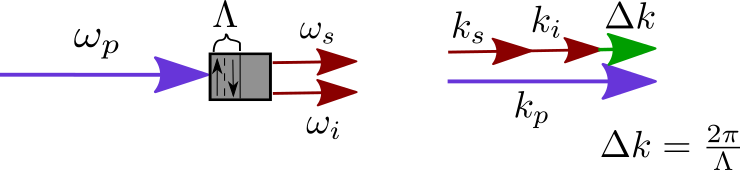
\includegraphics[width=6cm]{SPDCkQPM.png}}
		\end{center}
		%Conservation of momentum add here noob
		\label{fig:SPDCk}
	\end{figure}
	\tiny
	\begin{equation}
		I &\propto sinc^2\left(\frac{L \delta k}{2}\right)
		\label{eq:SPDCksinc2}
	\end{equation}
	\normalsize
\end{frame}

\begin{frame}[t]
	\frametitle{Theory}
	\framesubtitle{Polling}
	\begin{figure}
		\begin{center}
			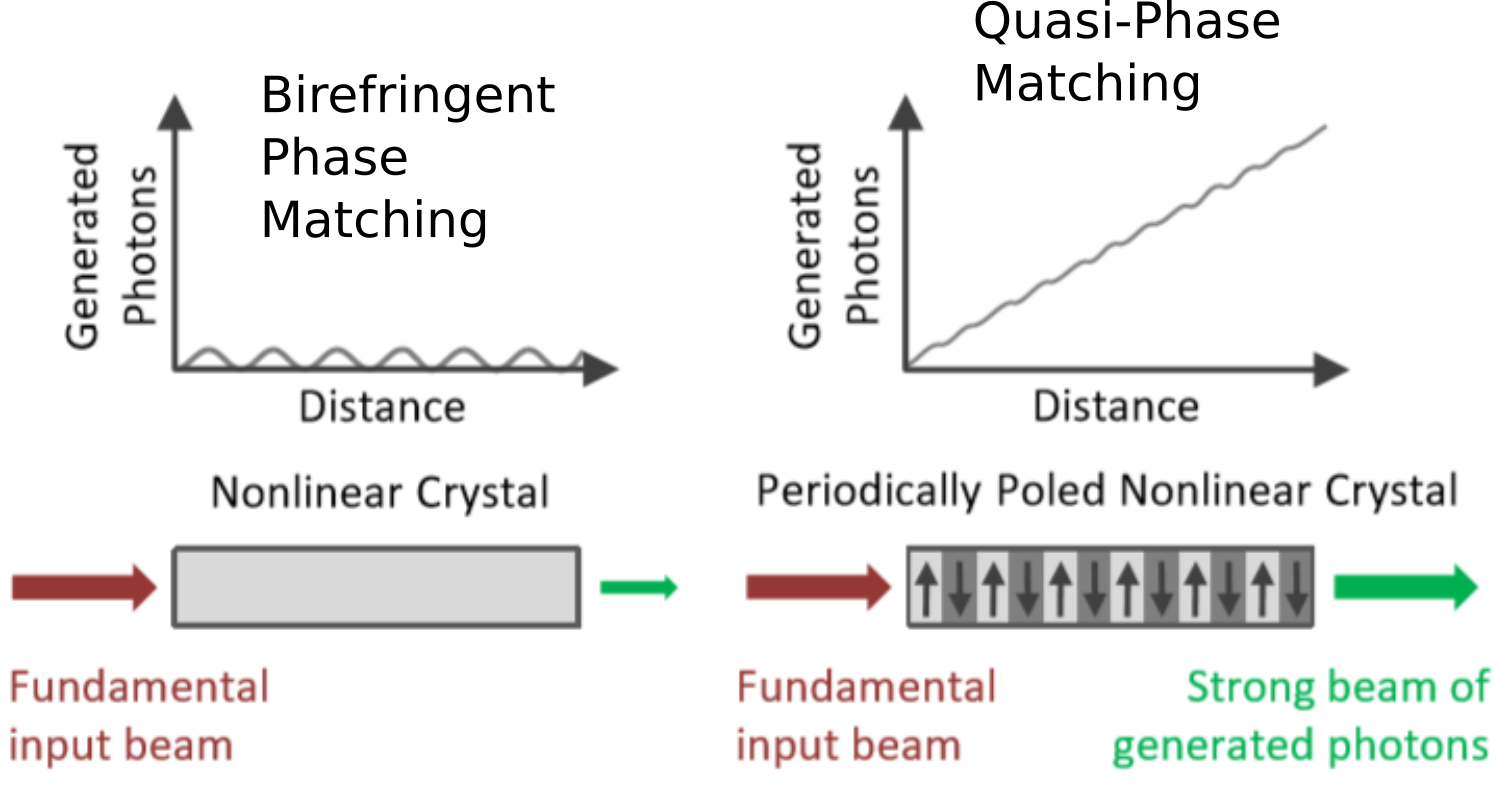
\includegraphics[width=10cm]{PolledVsNot.png}
		\end{center}
		\caption{Difference in photon generation between a unpolled and polled crystal.\\\textit{Source: RP-Photontics}}
		\label{fig:polledvsnot}
	\end{figure}
	
\end{frame}

\subsubsection{Phase Matching Temperature}
\begin{frame}{Theory}
	\framesubtitle{Phase Matching Temperature}
	\begin{figure}[!ht]
	  \centering
	  \caption{Phase Matching Temperature calculatios for a) Type-2 crystal of 9,12 $\mu$m polling period, b) Type-0, 19,25 $\mu$m, c) Type-0, 19,45 $\mu$m, d), Type-0 19,65 $\mu$m}
	  \subfloat[][]{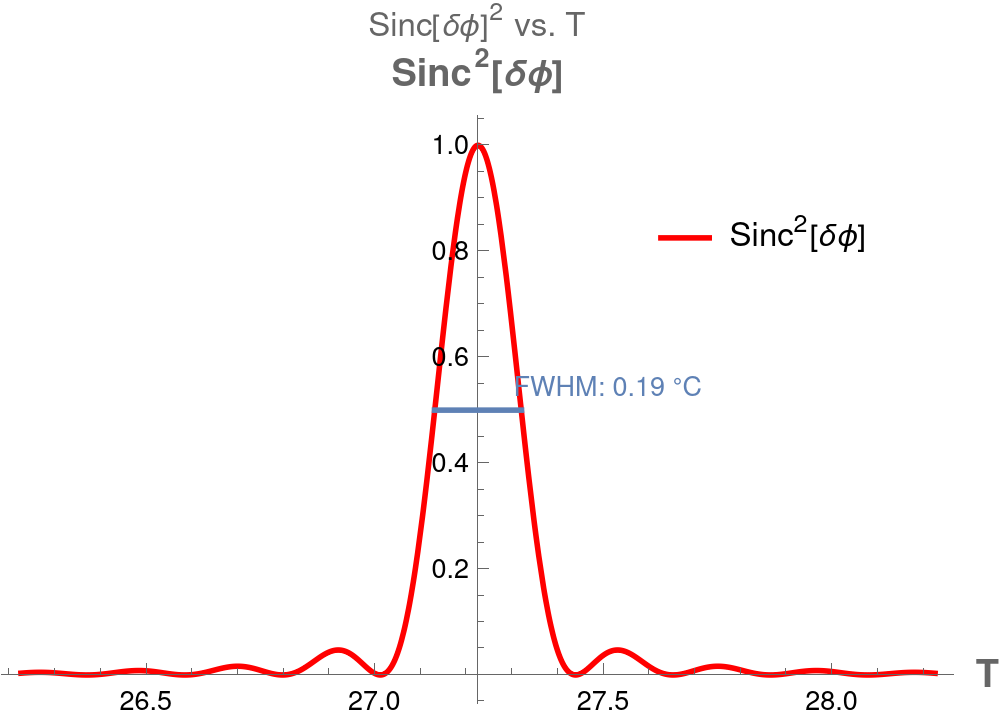
\includegraphics[width=3.9cm]{PMT_Type2.png}}\quad
	  \subfloat[][]{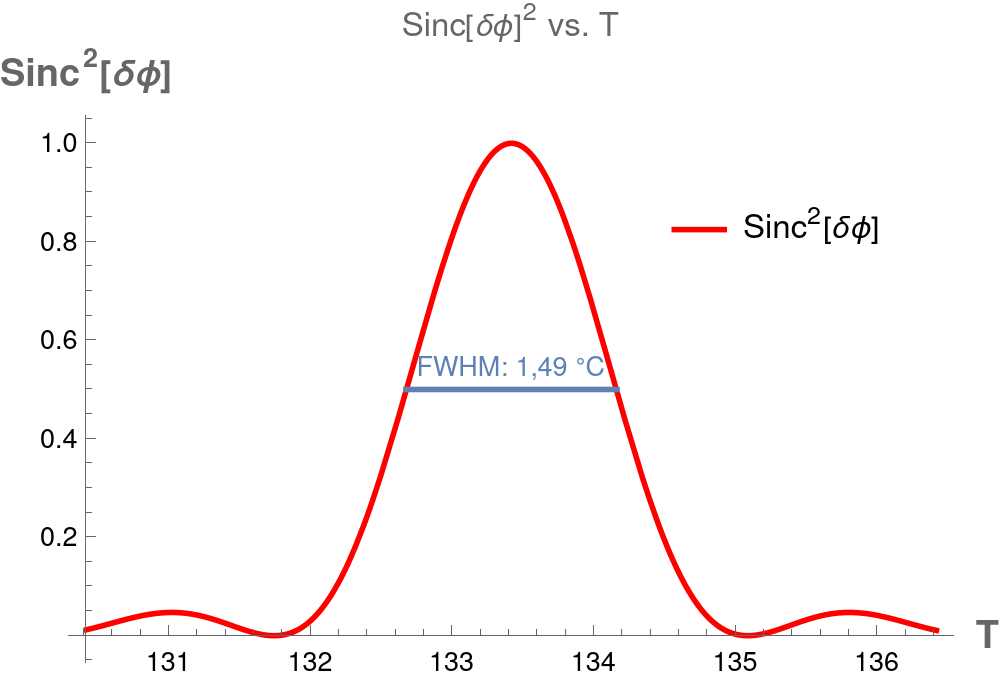
\includegraphics[width=3.9cm]{PMT_Type0G4.png}}\\
	  \subfloat[][]{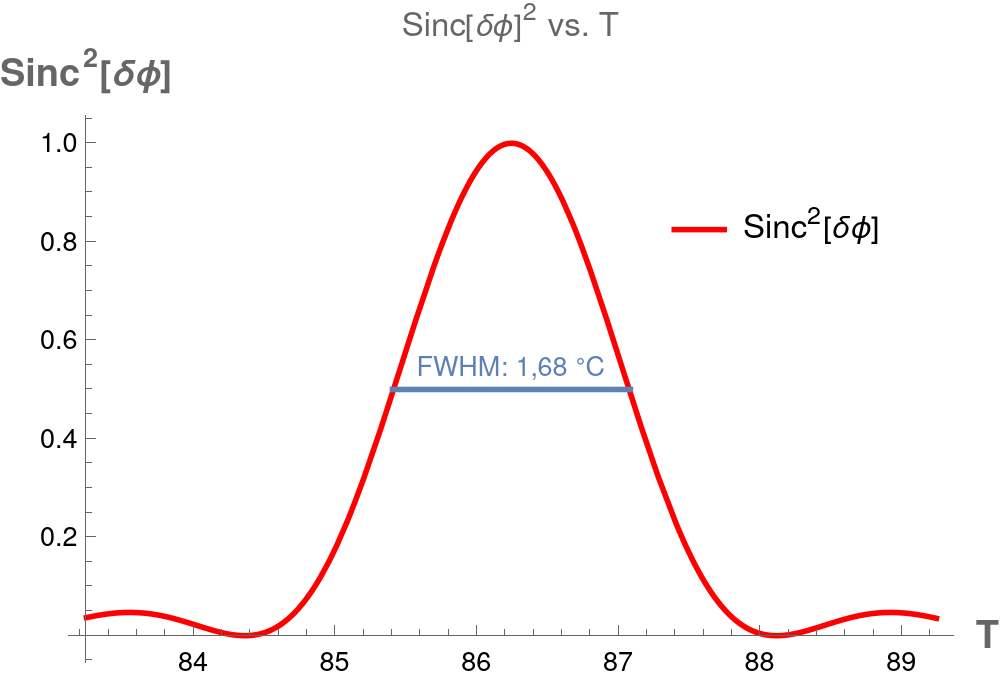
\includegraphics[width=3.9cm]{PMT_Type0G5.png}}\quad
	  \subfloat[][]{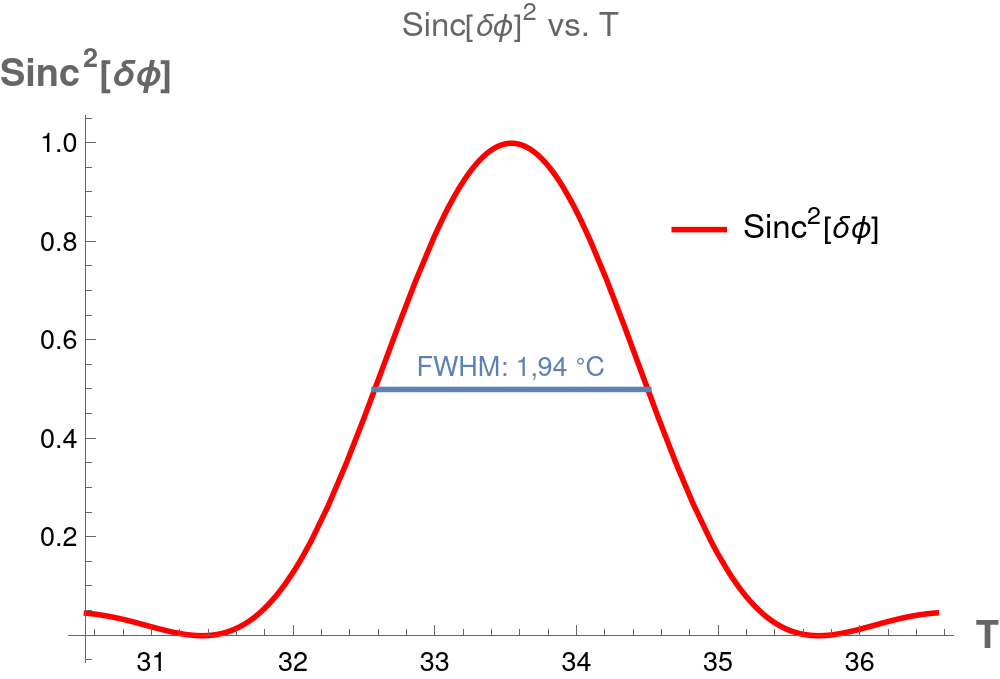
\includegraphics[width=3.9cm]{PMT_Type0G6.png}}\\
	  \label{fig:gratingstheory}
	\end{figure}
\end{frame}

\begin{frame}[t]
	\frametitle{Theory}
	\framesubtitle{Bandwidth}

	\begin{figure}[!ht]
	  \centering
	  \caption{Wavelength bandwidth of a) Type-2 crystal with a polling period of 9,12 $\mu$m\\ b) Type-0 crystals with polling periods of 19,25 $\mu$m}
	  % Do this on the same plot
	  \subfloat[][]{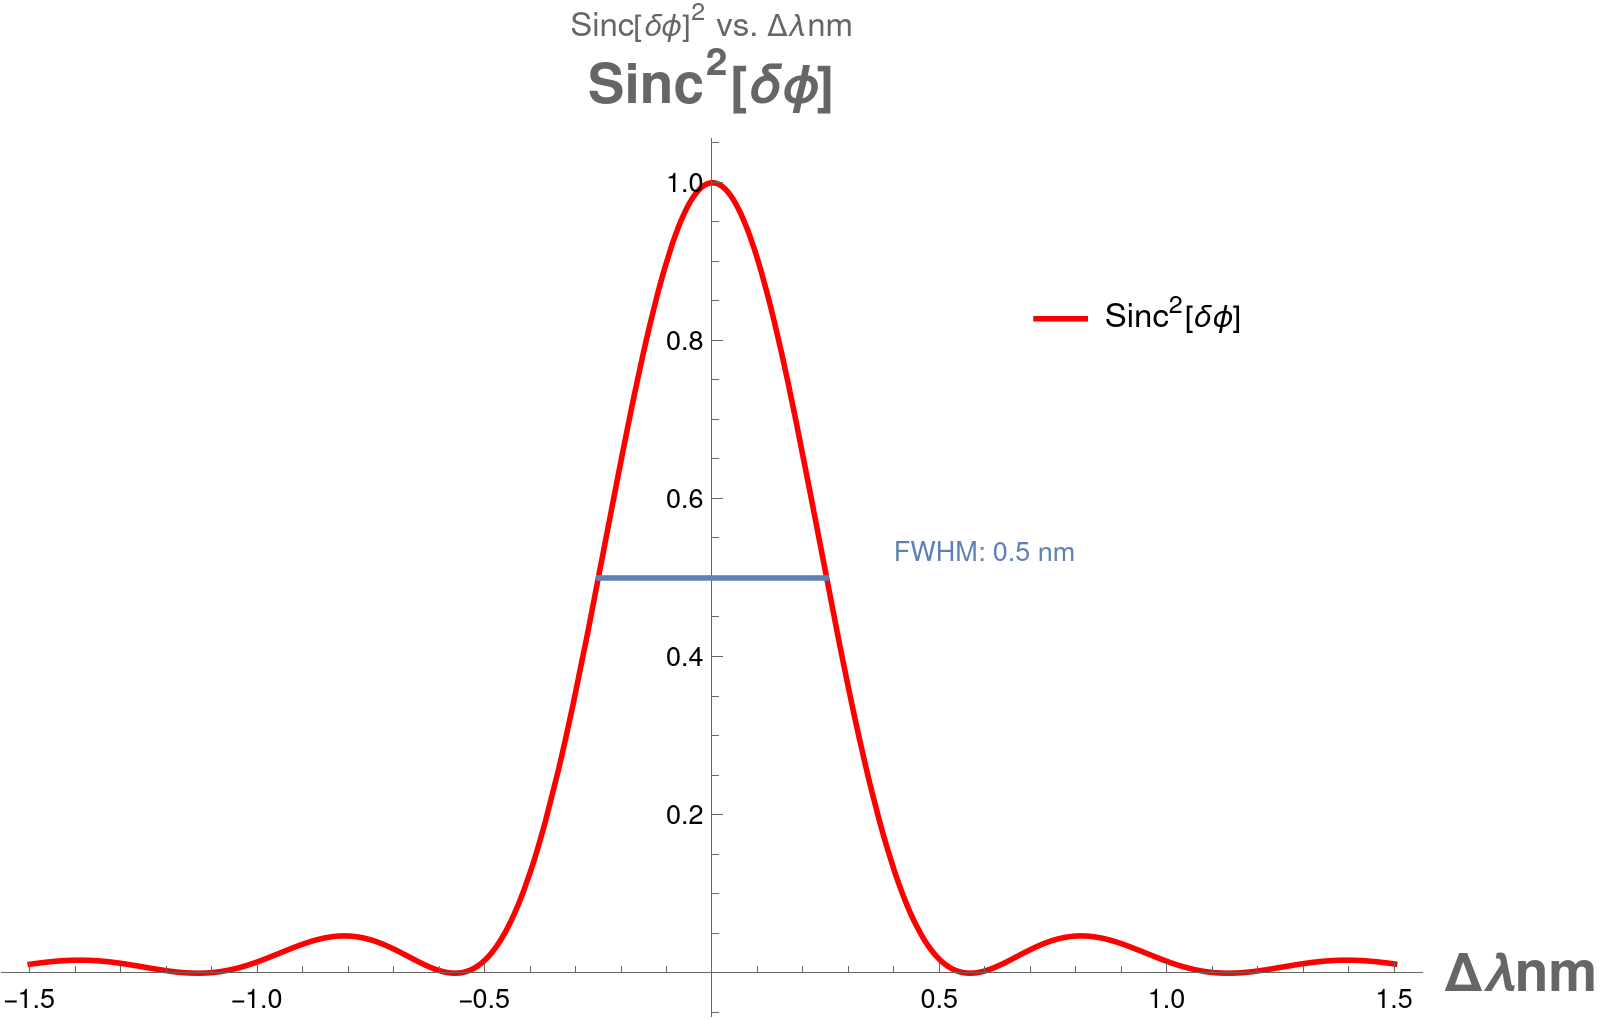
\includegraphics[width=5cm]{Type2wavelength.png}}\quad
	  \pause
	  \subfloat[][]{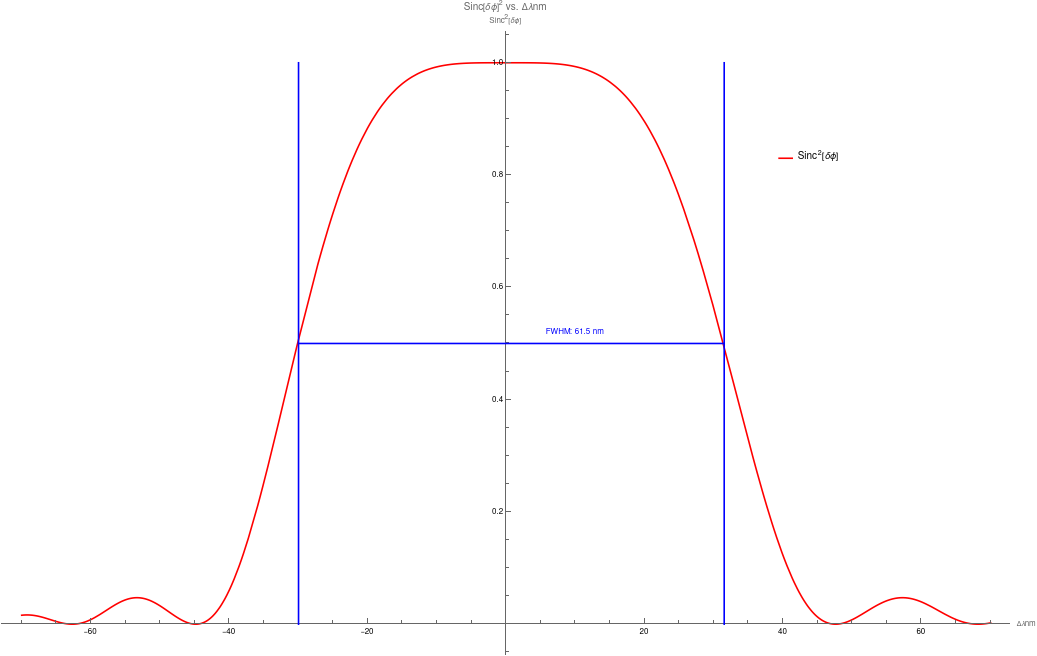
\includegraphics[width=5.5cm]{Type0wavelength.png}}
	  \label{fig:CompT0a2}
	\end{figure}
	\pause
	\tiny
	\begin{minipage}[t]{0.48\textwidth}
		\begin{equation}
		\begin{aligned}
			\ket{\Psi_{p}} &= \frac{1}{\sqrt{2}}(\sin(\alpha)a_{H}^{\dagger}+\cos(\alpha)a_{V}^{\dagger})\ket{0}\\
			\ket{\Psi_{\text{Type-2}}} &= \frac{1}{\sqrt{2}}(\sin(\alpha)a_{H}^{\dagger}(\omega_s)a_{V}^{\dagger}(\omega_i)+\\
								&\cos(\alpha)a_{V}^{\dagger}(\omega_i)a_{H}^{\dagger}(\omega_s))\ket{0}\\
		\end{aligned}
		\end{equation}
	\end{minipage}
	\begin{minipage}[t]{0.48\textwidth}
	\begin{equation*}
		\begin{aligned}
			\ket{\Psi_{\text{Type-0}}} &= \frac{1}{\sqrt{2}}(\sin(\alpha)a_{H}^{\dagger}(\omega_s)a_{H}^{\dagger}(\omega_i)+\\
									   &\cos(\alpha)a_{V}^{\dagger}(\omega_i)a_{V}^{\dagger}(\omega_s))\ket{0}
		\end{aligned}
	\end{equation*}
	\end{minipage}
	\normalsize
\end{frame}

\begin{frame}
	\frametitle{Theory}
	\framesubtitle{Current brightness between FMF and IJS}
	\begin{table}
		\begin{center}
			\caption{Current brightness estimation [$\frac{Hz}{mWnm}$]}
			\begin{tabular}[c|c|c]{|ll|l|}
				\hline
				\multicolumn{1}{|c}{\hfill\textbf{FMF}\hfill} &&
				\multicolumn{1}{c|}{\textbf{IJS}} \\
				\hline
				\multicolumn{1}{|c|}{\textbf{Type-II}} &
				\multicolumn{1}{c|}{\textbf{Type-0}} &
				\multicolumn{1}{c|}{\textbf{Type-II}} \\
				\hline
				7,8 $\times10^6$ & 2,6 $\times 10^7 $ & 0,05 $\times 10^6$ \\
				\hline
				\multicolumn{1}{|c}{\textbf{Bandwidth} [ nm ]} &\multicolumn{1}{c}{ } & \multicolumn{1}{c|}{ }  \\
				\hline
				0,81 & 0,81 & 0,81\\
				\hline
			\end{tabular}
		\end{center}
	\end{table}
	% Overestimated for the "bad" detectors - One has to take into account the dead-time maybe so maybe no one is doing this correctly? :P
\end{frame}

%	TODO: DO THIS ALREADY YOU IDIOT
% \subsubsection{Efficiency}
% \begin{frame}
% 	\frametitle{SPDC}
% 	\framesubtitle{Expected efficiency}
% 	Fiorentino Expected efficiency
% 	Might not be important
% \end{frame}


%	TODO: DO THIS ALREADY
% \subsubsection{Detectors}
% \begin{frame}
% 	\frametitle{Detectors}
% 	\framesubtitle{Dependence of detector dead-time and efficiency}
% 	\Huge Most important
% 	\large
% Dead-time dependency
% \end{frame}

\begin{frame}[t]
	\frametitle{Different Designs}
	\begin{figure}[!ht]
	  \centering
	  \caption{Different design ideas from other groups. a) \cite{design4}, b) \cite{design1}, c) \cite{design3}, d) \cite{design2}}
	  \subfloat[][]{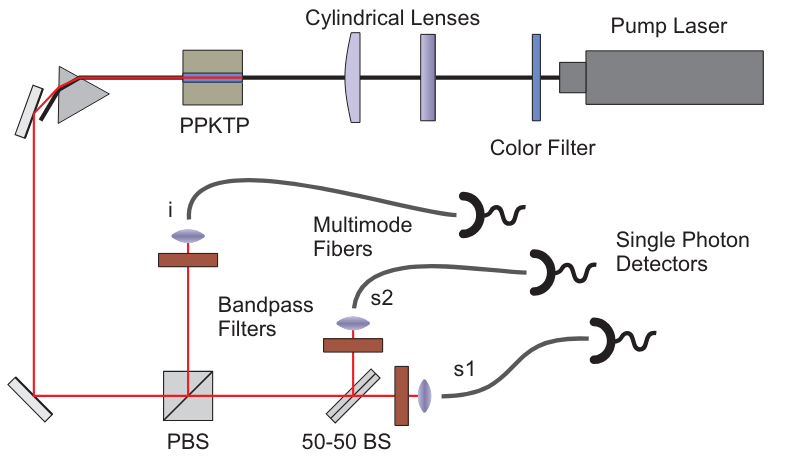
\includegraphics[width=5cm]{Design4.png}}\quad
	  \subfloat[][]{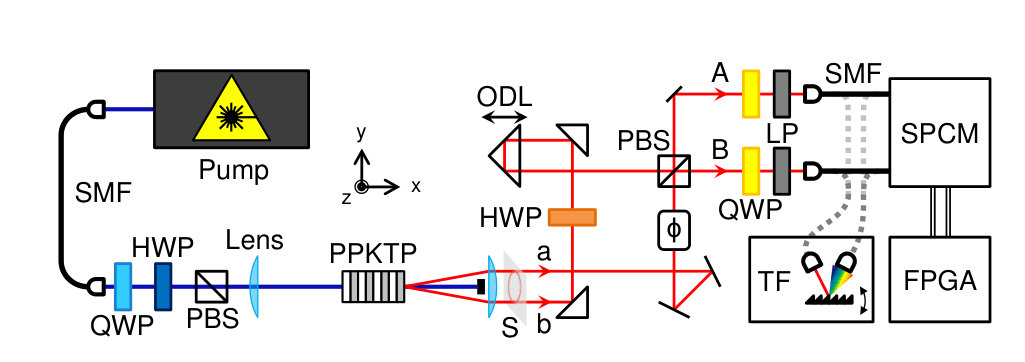
\includegraphics[width=5cm]{Design1.png}}\\
	  \subfloat[][]{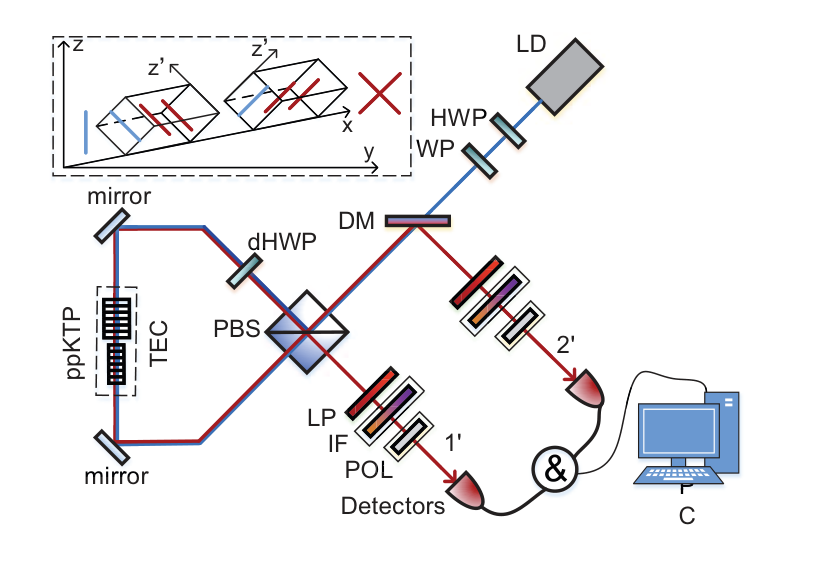
\includegraphics[width=4cm]{Design3.png}}\quad
	  \subfloat[][]{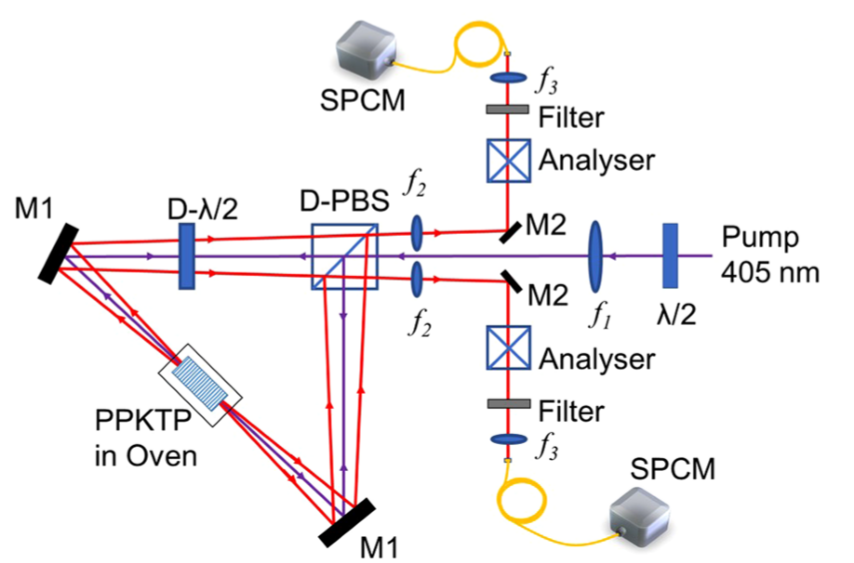
\includegraphics[width=4.5cm]{Design2.png}}\\
	  \label{fig:sub4}
	\end{figure}
\end{frame}

\subsection{Distributing Entanglement}
\begin{frame}[t]
	\frametitle{Why do we care about entanglement?}
	\begin{itemize}
		\item Entanglement sources by themselves $\rightarrow$ usless if you can't use them.
		\item Loss in fiber
	\end{itemize}
	\begin{table}
		\caption{Relevant fiber loss.\\\textit{Source: Thorlabs}}\label{tab:fiberloss}
		\begin{tabular}{|c|c|c|}
			\hline
			$\lambda$ [nm] & 1310 & 1550\\
			\hline
			Loss [dB/km] & 0.32 &  0.18\\
			\hline
		\end{tabular}
	\end{table}
	\begin{exampleblock}{Example: Loss in fiber for 1550/1560 nm}
		200 km of fiber \rightarrow $10^4$ loss.
	\end{exampleblock}
	\begin{figure}
		\begin{center}
			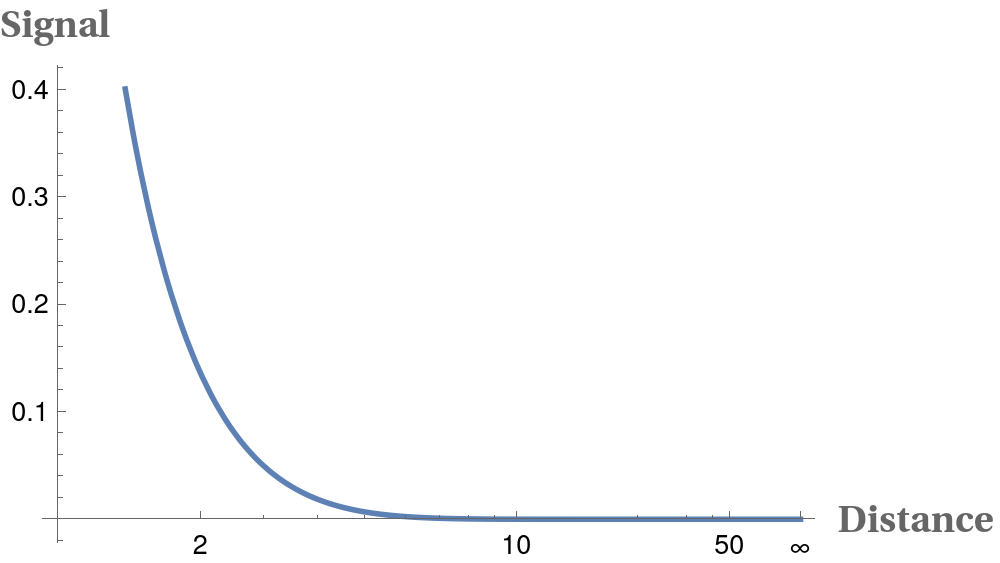
\includegraphics[width=7cm]{FiberLoss.png}
		\end{center}
		\caption{Loss in fiber over distance.}\label{fig:fiberloss}
	\end{figure}
	
\end{frame}

\begin{frame}{Distributing Entanglement}
	\framesubtitle{Introduction}
	\begin{itemize}
		\item No specific form required - arbitrary states can be teleported
			%	TODO: Make a graphic of this
			%	Two pairs of maximally entangled qubits.
			%	Pair one = qubit 1 and qubit 2
			%	Pair two = qubit 3 and qubit 4
			%	Teleport qubit 2: Perform Bell State Measurement on qubit 2 and qubit 3
			%	If teleportation + success == true -> qubit 2 and qubit 3 states are destroyed (no-cloning theorem) -> Qubit 1 and Qubit 4 now in same entangled state
			\begin{enumerate}
				% QUANTUM REPEATERS IN HANDWAVEY WAY
				\item Bell State Measurements
				\item Will try to use Quantum Memory from IJS group
			\end{enumerate}
			% NOTE: Distillation and repeaters - Rainer PhD ----
		\item FMF/IJS
		\item Government buildings in Ljubljana
	\end{itemize}
\end{frame}

\subsubsection{Entanglement Teleportation}
\begin{frame}[t]
    \frametitle{Entanglement Teleportation}
    \framesubtitle{Teleportation}
    \begin{figure}[]
      \centering
      \caption{Illustration of Entanglement Teleportation.}
      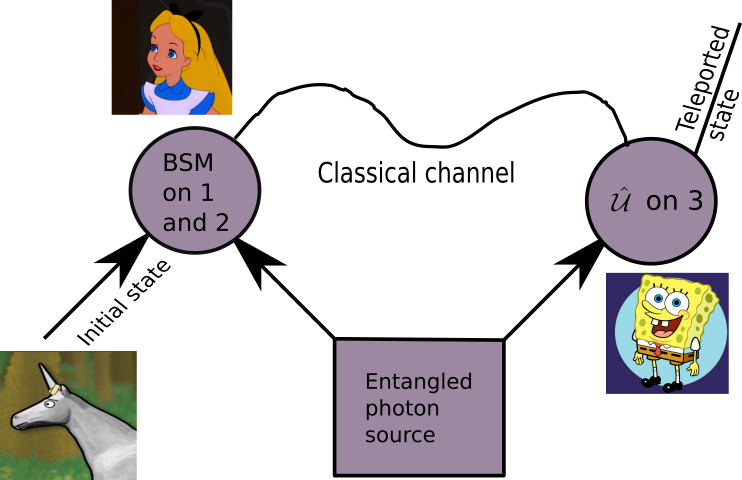
\includegraphics[width=8cm]{EntanglementTeleportation.png}
	\label{fig:Tele}
    \end{figure}
\end{frame}

%add image for the 50% case -> PBS after BS


\subsubsection{Entanglement Swapping}
\addtocounter{framenumber}{-1}
\begin{frame}[t]
    \frametitle{Entanglement Swapping}
    \framesubtitle{Swapping}
\begin{figure}[]
      \centering
      \caption{Illustration of Entanglement Swapping.}
      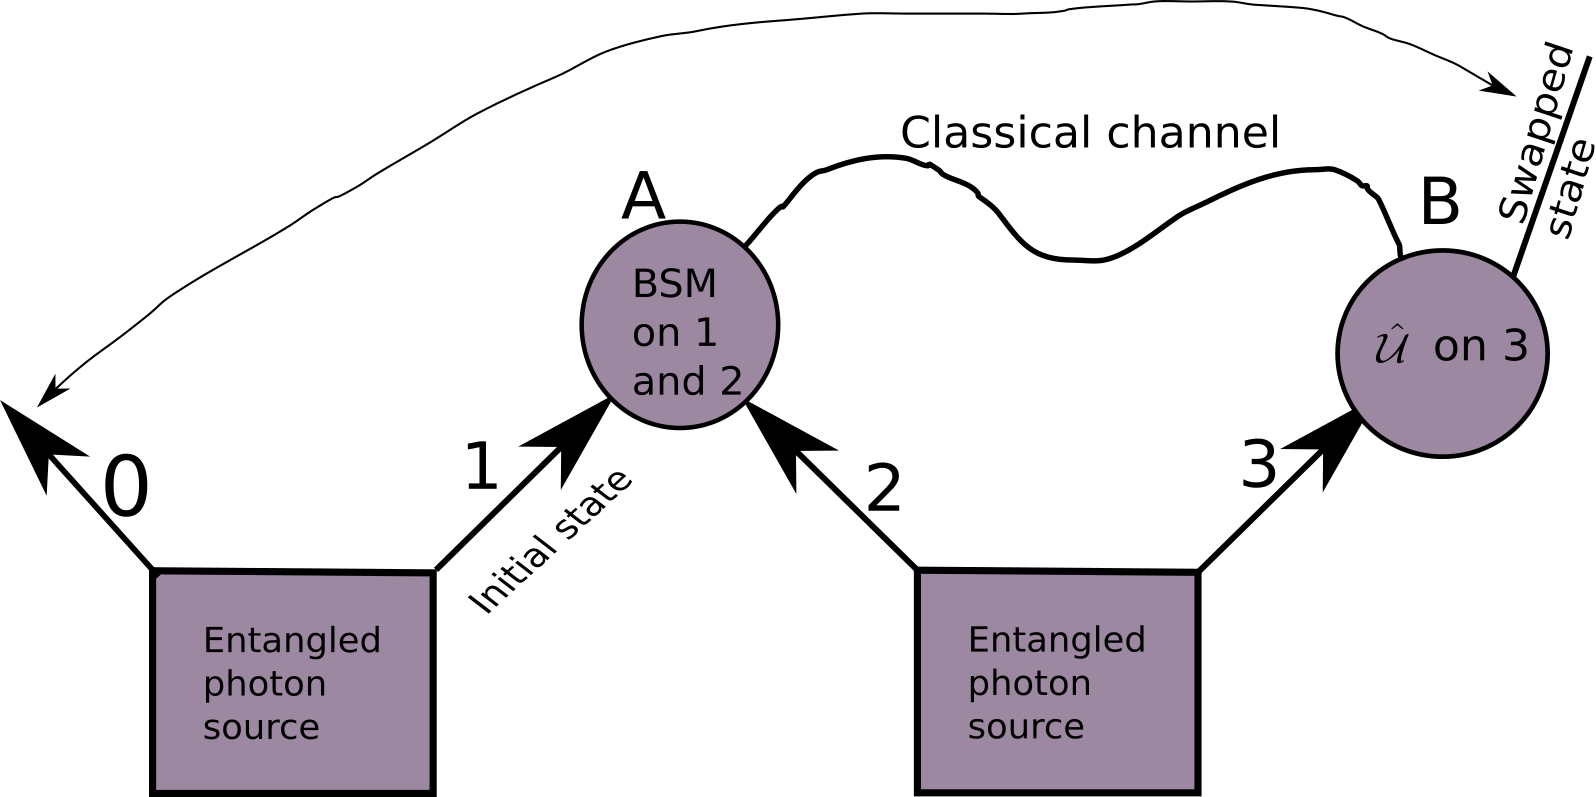
\includegraphics[width=10cm]{EntanglementSwapping.png}
	\label{fig:Swap}
    \end{figure}
\end{frame}

\section{Present state}

\subsection{Parameters}
\begin{frame}[t]
	\frametitle{Present state}
	\framesubtitle{Parameters}
		\begin{itemize}
			\item Focusing parameters \cite{bennik}
					\begin{equation}
							\xi = \frac{L}{k w^2}
						\label{eq:Focusing parameter}
					\end{equation}\\
					Photon generation
			\item Correct lenses and distances for efficient coupling
			\item Correct size of coupler apperture
		\end{itemize}

	\begin{figure}[!ht]
	  \centering
	  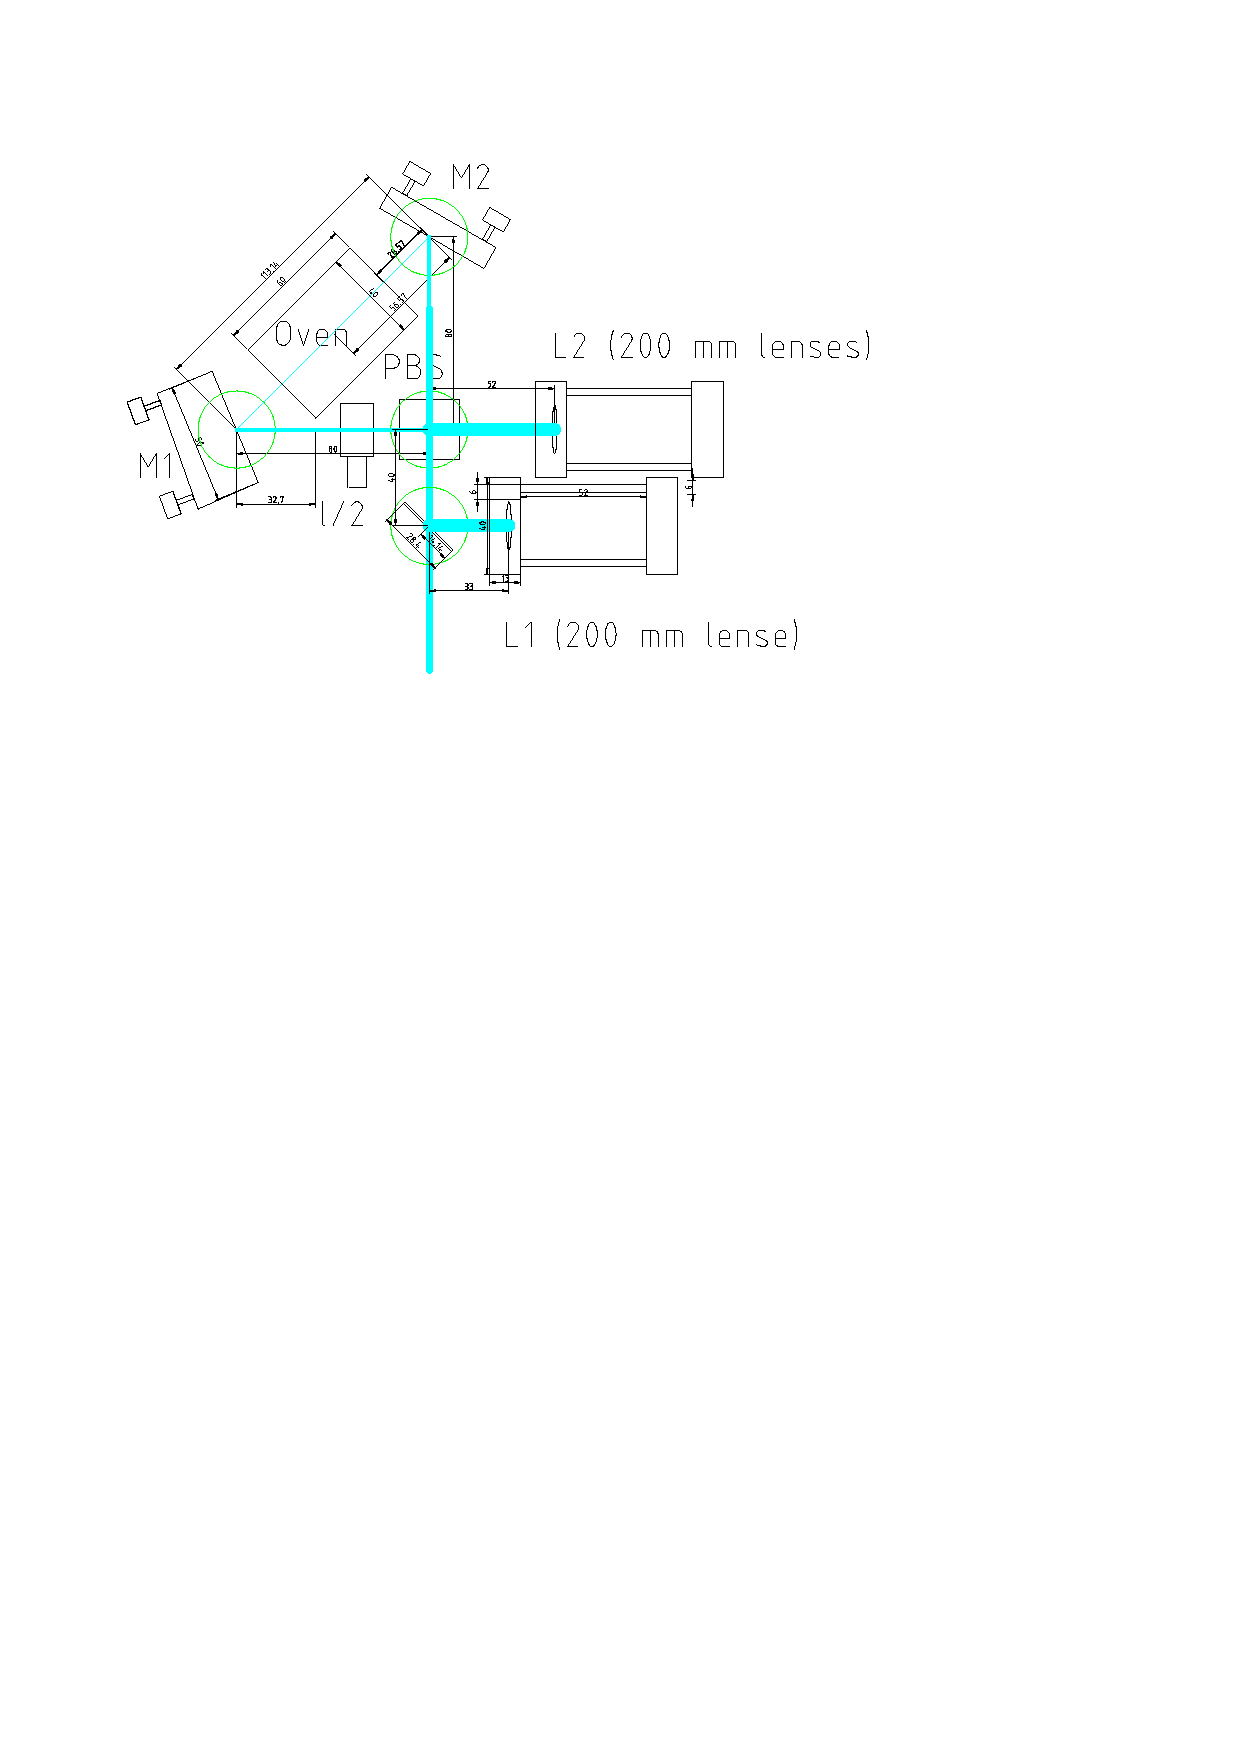
\includegraphics[angle=90,width=7cm]{SagnacDesign.pdf}
	  \caption{Design of the Sagnac interferometer.}
	\end{figure}
\end{frame}

\subsection{Phase Matching Temperature}
%Temperatures in the 100°C-200°C range are used in order to minimize the photorefractive effect that can damage the crystal and causes the output beam to be distorted.
%Since the photorefractive effect is more severe in PPLN when higher energy photons in the visible part of the spectrum are present in the crystal,
%it is especially important to use the crystal only in the recommended temperature range.
%When using a PPLN crystal as an OPO that is pumped with and generates light in the infrared region of the spectrum,
% it may be possible to use temperatures lower than 100°C if necessary without damaging the crystal.
\begin{frame}{Present state}
	\framesubtitle{Phase Matching Temperature}
	\begin{figure}[!ht]
	  \centering
	  \caption{Temperature scans of Type-0 crystals with different polling periods, a) misaligned 19,25 $\mu$m, b) 19,25 $\mu$m, c) 19,45 $\mu$m, d) 19,65 $\mu$m}
	  % TODO: HAVE TO MAKE THIS BIGGER INCREASE TEXT SIZE IN PYTHON FUCKING NOOB
	  \subfloat[][]{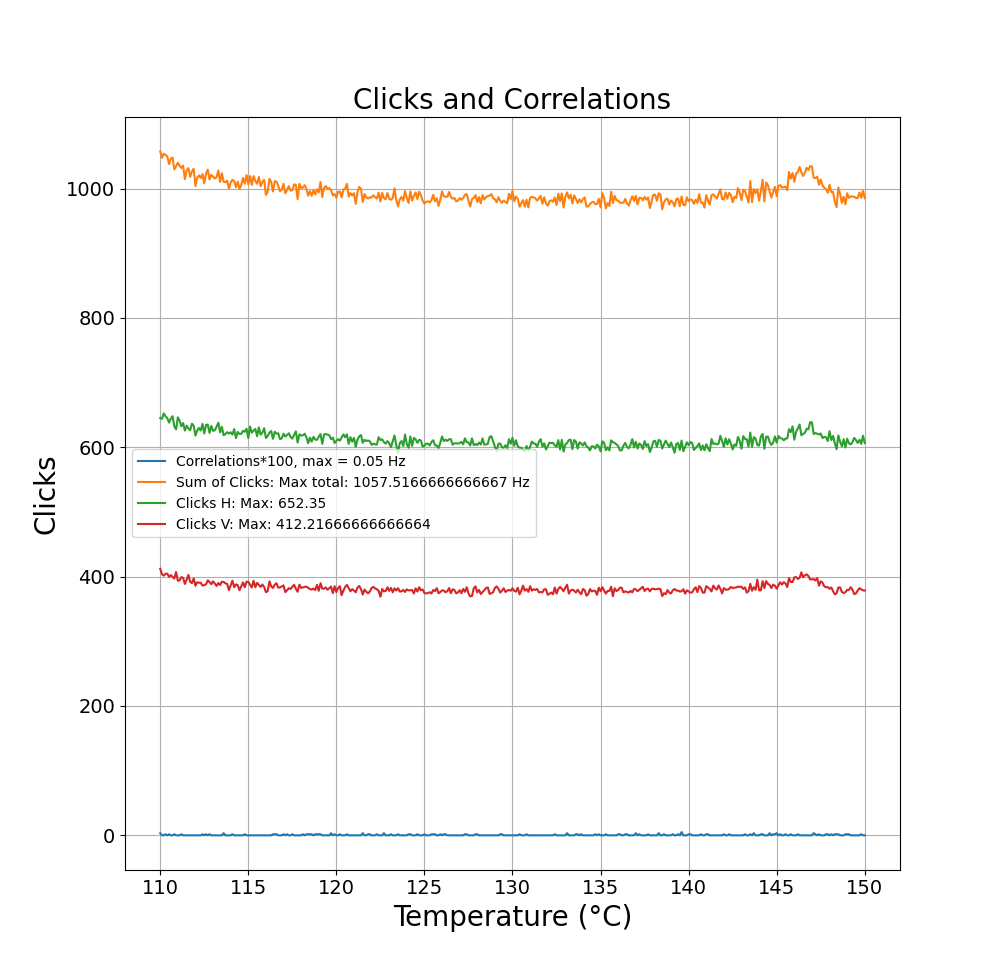
\includegraphics[width=2.9cm]{Not_Aligned_Scan.png}}\quad
	  \subfloat[][]{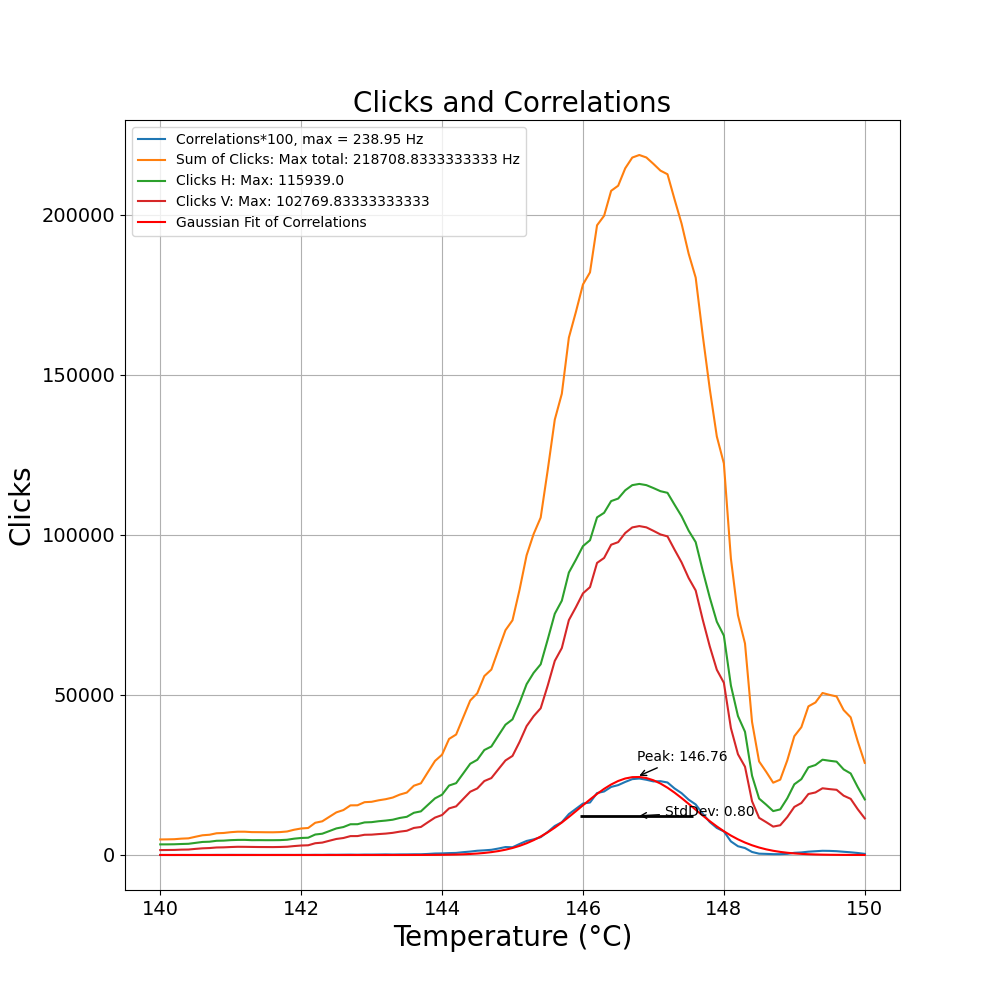
\includegraphics[width=2.9cm]{PMT_Grating_4.png}}\\
	  \subfloat[][]{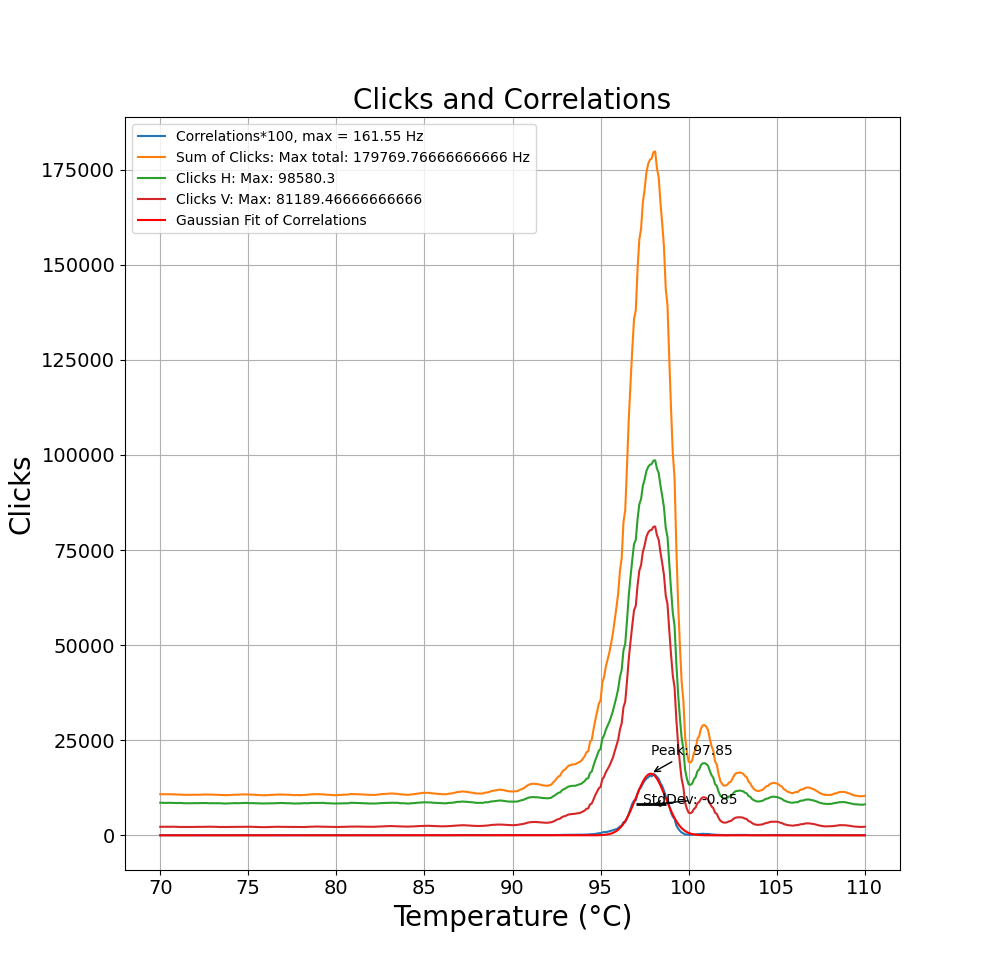
\includegraphics[width=2.9cm]{PMT_Grating_5.png}}\quad
	  \subfloat[][]{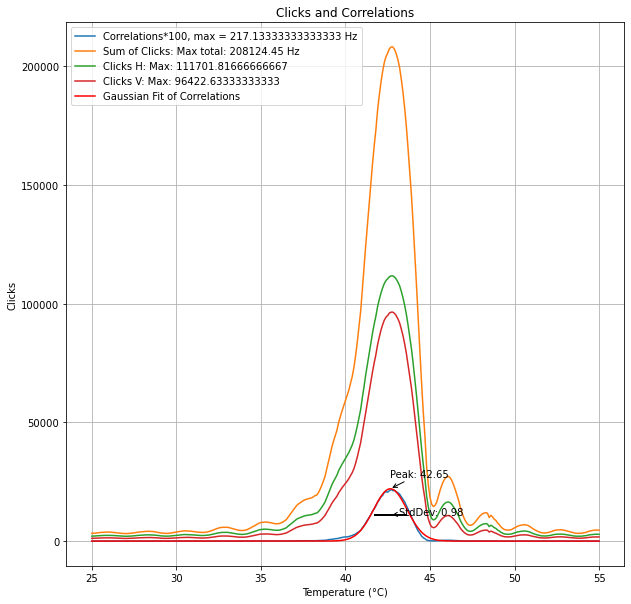
\includegraphics[width=2.9cm]{PMT_Grating_6.png}}\\
	  \label{fig:gratings}
	\end{figure}
\end{frame}

\subsection{Building a Sagnac Interferometer}
{\usebackgroundtemplate{\includegraphics[width=\paperwidth,height=\paperheight]{SagnacWithSomeAddedColoursV1.png}}

\begin{frame}[t]
	\frametitle{Present state}
	\framesubtitle{Building a Sagnac Interferometer}
	\begin{figure}[!ht]
	  \centering
	  \pause
	  \subfloat[][]{\includegraphics[width=8cm]{Type0Gratings.pdf}}\\
	  \caption{\textcolor{white}{Specifications from the crystal manufacturer.\\\textit{Source: HC Photonics Corp.}}}
	\end{figure}
\end{frame}

\usebackgroundtemplate{}
\section{Outlook}
\begin{frame}{Outlook}
	\begin{itemize}
		\item SiQUID
		\item Entanglement swapping between FMF and IJS
		\item Building quantum network
		\item Free space link to reactor
	\end{itemize}
	% Entanglement swapping over short distance, IJS, Reactor with fibers, take one of the sources and do Entanglement swapping over long distances
\end{frame}

\addtocounter{framenumber}{-1}
\begin{frame}[plain]{\ }
	\begin{center}
	\Huge
	Thank you
	\end{center}
\end{frame}


\addtocounter{framenumber}{-1}
\begin{frame}[plain]
	\frametitle{References}
	\tiny
	\bibliographystyle{IEEEtran}
	\bibliography{reference}
\end{frame}

\end{document}
